% Hypnagogia: a pre-registered test for offline memory replay in a
% whole-brain Drosophila connectome model.
% Build: tectonic hypnagogia.tex   (XeTeX; runs BibTeX automatically)

\documentclass[11pt]{article}

% ---------------------------------------------------------------- layout
% Matches the Agentical paper's format: plain article, Computer Modern,
% numbered natbib citations, hidden links, default captions and headings.
\usepackage[T1]{fontenc}
\usepackage{amsmath, amssymb, mathtools}
\usepackage{xcolor}
\usepackage{geometry}
\usepackage{microtype}
\usepackage{booktabs}
\usepackage{array}
\usepackage{tabularx}
\usepackage[inline]{enumitem}
\usepackage[numbers,sort&compress]{natbib}
\usepackage{tikz}
\usetikzlibrary{arrows.meta,positioning,fit,calc}
\usepackage{pgfplots}
\pgfplotsset{compat=1.18}
\usepackage[hidelinks]{hyperref}

\geometry{margin=1in}
\setlength{\emergencystretch}{3em}

% table captions sit above the table, so the gap belongs below the caption
\let\origtable\table
\renewcommand{\table}{\setlength{\abovecaptionskip}{0pt}\setlength{\belowcaptionskip}{6pt}\origtable}

% figure tones: black and greys only, as in the Agentical figures
\definecolor{accent}{gray}{0.15}
\definecolor{edge}{gray}{0}
\definecolor{quiet}{gray}{0.2}
\newcolumntype{L}{>{\raggedright\arraybackslash}X}

\newcommand{\Dm}{\emph{Drosophila}}
\newcommand{\KCMBON}{KC$\rightarrow$MBON}

% ---------------------------------------------------------------- title
\title{%
  Hypnagogia: A Pre-Registered Test for Offline Memory Replay \\
  in a Whole-Brain \emph{Drosophila} Connectome Model
}

\author{
  Aniketh Bandlamudi \\
  \small University of Virginia \\
  \small\texttt{zpq3uh@virginia.edu}\quad\texttt{me@aniketh.net}
}

\date{November 2026}

\begin{document}
\maketitle

\begin{abstract}
\noindent Sleep replay of learned activity is well described in the rodent hippocampus, but offline reactivation of a learned ensemble has never been observed in an insect. We asked whether a whole-brain leaky integrate-and-fire model of the \Dm{} male central brain connectome (144,209 neurons, 21.9 million connections), built on the model of \citet{shiu2024}, reactivates a learned Kenyon-cell ensemble during simulated sleep. Our reimplementation reproduced the published model on its own data (per-neuron rate correlation $r = 0.9997$). We then corrected two mushroom-body cells against direct measurements, adding no parameter: APL became a non-spiking, graded-release neuron and DPM became inhibitory. The APL correction alone moved odour coding from 52.6\% of Kenyon cells at 23.0~Hz to 4.5\% at 0.79~Hz, against $6 \pm 5\%$ measured in flies. An odour memory was encoded by dopamine-gated depression at Kenyon-cell-to-output-neuron synapses and tested against four pre-registered comparisons over 20 seeds. The test failed. The memory changed offline Kenyon-cell activity in all 20 seeds and reduced drive through the learned synapses by 32.5\%, but it did not increase reactivation of the trained ensemble (learned minus unlearned weights: $+0.016$, 95\% CI $-0.011$ to $+0.044$). An injected positive control showed that the published model cannot hold a discrete episode. Adding spike-frequency adaptation, a labelled deviation, produced episodes and a sparser code, yet the memory still contributed nothing ($+0.040$, 95\% CI $-0.010$ to $+0.090$). The model's only plastic synapses sit downstream of the cells being scored, and the path back delivers under 1\% of a threshold gap even at 50~Hz. Kenyon-cell replay is therefore a question this model class cannot answer positively; the negative is a finding about the model, not about the fly.

\end{abstract}

\tableofcontents
\newpage

% =====================================================================
\section{Introduction}

In the rat hippocampus, ensembles that fire together during waking fire together again during later sleep \citep{wilson1994,kudrimoti1999}. During pauses in waking behaviour, place cells can also replay the order in which they fired, in reverse \citep{foster2006}. Offline reactivation of a learned ensemble, above chance and above structural controls, has become the standard operational test for replay.

The fly has the ingredients for the same question but no answer to it. Activating dorsal fan-shaped body (dFB) neurons promotes sleep \citep{donlea2014,pimentel2016}, and R5 ring neurons show network-generated up and down states at 0.5 to 1.5~Hz whose power rises with sleep need \citep{raccuglia2019}. The mushroom body stores odour memories: Kenyon cells code odours sparsely, about $6 \pm 5\%$ of cells per odour \citep{turner2008,honegger2011}, and dopamine-gated depression at Kenyon-cell-to-output-neuron (\KCMBON{}) synapses writes the association \citep{hige2015}. Sleep supports memory consolidation in flies \citep{haynes2015,berry2015}, and dopaminergic neurons active during training are reactivated in post-learning sleep, as read out by a transcriptional reporter over hours \citep{dag2019}. Yet offline reactivation of a Kenyon-cell ensemble has never been observed in a real fly, and the fly has no described analogue of the hippocampal sharp-wave ripple that organises mammalian replay.

Whole-brain connectomes make it possible to ask the question in simulation. \citet{shiu2024} built a leaky integrate-and-fire (LIF) model of every neuron in the FlyWire connectome \citep{dorkenwald2024} and showed that it predicts sensorimotor pathways for taste. The male central nervous system (CNS) connectome v1.0 \citep{berg2026} now provides a second complete, proofread brain. A model built on it lets replay be tested as a controlled experiment: the same network with and without learning, with real and shuffled wiring, in sleep and in wake.

This paper reports that experiment, a project we call Hypnagogia. Its contributions are:
\begin{enumerate}\setlength\itemsep{1pt}
  \item a Brian2 reimplementation of the \citet{shiu2024} model that reproduces the published output, ported to the male CNS connectome and validated there;
  \item two corrections to mushroom-body cells that the published model mis-specifies, each taken from a direct measurement and adding no parameter, of which the APL correction is the largest single effect in the project;
  \item a pre-registered replay test with four required comparisons and an unlearned-weights control, run over 20 seeds, which is negative;
  \item a diagnosis of the negative: the model cannot hold an episode, the memory is expressed tonically rather than in episodes, and the only plastic synapses sit downstream of the cells being scored;
  \item a demonstration that adding a slow variable produces episodes but still no replay.
\end{enumerate}
Every number below is read from the project's result files. Departures from the published model are labelled as deviations wherever they appear, and any constant without a measurement behind it is scanned rather than chosen.

% ---------------------------------------------------------------- Fig 1
\begin{figure}[t]
\centering
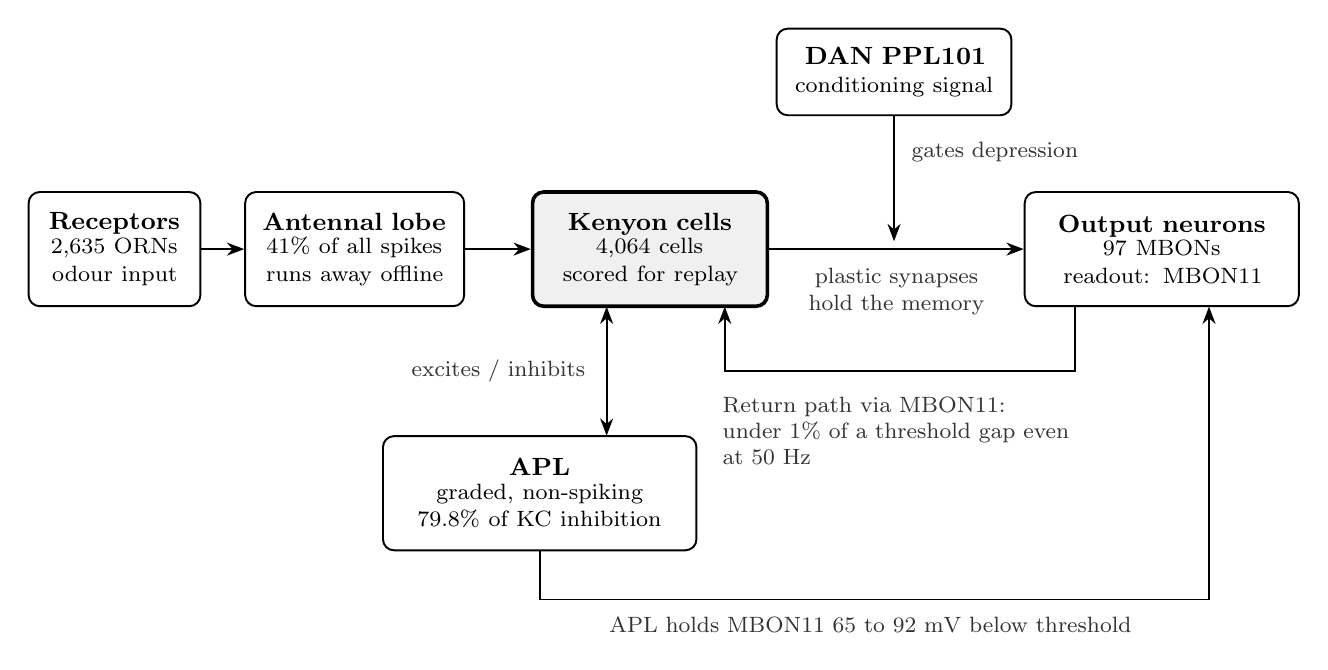
\begin{tikzpicture}[
  font=\small,
  box/.style={draw=edge, rounded corners=4pt, line width=0.7pt, align=center, minimum height=1.45cm, inner sep=4pt},
  main/.style={box, draw=black, line width=1.3pt, fill=gray!12},
  arr/.style={-{Stealth[length=2.2mm]}, draw=edge, line width=0.7pt},
  lab/.style={font=\footnotesize, text=quiet, align=left}
]
  \node[box, text width=1.9cm] (orn) at (0,0) {\textbf{Receptors}\\[-1pt]\footnotesize 2,635 ORNs\\[-1pt]\footnotesize odour input};
  \node[box, text width=2.5cm] (al)  at (3.05,0) {\textbf{Antennal lobe}\\[-1pt]\footnotesize 41\% of all spikes\\[-1pt]\footnotesize runs away offline};
  \node[main, text width=2.7cm] (kc) at (6.8,0) {\textbf{Kenyon cells}\\[-1pt]\footnotesize 4,064 cells\\[-1pt]\footnotesize scored for replay};
  \node[box, text width=3.2cm] (mb)  at (13.3,0) {\textbf{Output neurons}\\[-1pt]\footnotesize 97 MBONs\\[-1pt]\footnotesize readout: MBON11};
  \node[box, text width=2.7cm, minimum height=1.1cm] (dan) at (9.9,2.25) {\textbf{DAN PPL101}\\[-1pt]\footnotesize conditioning signal};
  \node[box, text width=3.7cm] (apl) at (5.4,-3.1) {\textbf{APL}\\[-1pt]\footnotesize graded, non-spiking\\[-1pt]\footnotesize 79.8\% of KC inhibition};

  \draw[arr] (orn) -- (al);
  \draw[arr] (al) -- (kc);
  \draw[arr] (kc) -- (mb);
  \draw[arr] (dan.south) -- ($(dan.south |- kc.east)+(0,0.1)$);
  \node[lab, anchor=west] at ($(dan.south)+(0.1,-0.45)$) {gates depression};
  \node[lab, align=center, anchor=north] at ($(kc.east)!0.5!(mb.west)+(0,-0.12)$) {plastic synapses\\hold the memory};

  % KC <-> APL feedback
  \draw[{Stealth[length=2.2mm]}-{Stealth[length=2.2mm]}, draw=edge, line width=0.7pt] (6.25,-0.73) -- (6.25,-2.37);
  \node[lab, anchor=east] at (6.1,-1.55) {excites / inhibits};

  % return path MBON -> KC
  \draw[arr] (12.2,-0.73) -- (12.2,-1.55) -- (7.75,-1.55) -- (7.75,-0.73);
  \node[lab, anchor=north west, text width=4.4cm, execute at begin node={\hyphenpenalty=10000}] at (7.6,-1.75) {Return path via MBON11: under 1\% of a threshold gap even at 50~Hz};

  % APL silences MBON11
  \draw[arr] (5.4,-3.83) -- (5.4,-4.45) -- (13.9,-4.45) -- (13.9,-0.73);
  \node[lab, anchor=north] at (9.6,-4.55) {APL holds MBON11 65 to 92 mV below threshold};
\end{tikzpicture}
\caption{The memory sits one synapse downstream of the cells scored for replay. Learning depresses \KCMBON{} synapses, gated by the conditioning dopaminergic neuron PPL101. The engram can reach the Kenyon cells only through MBON11's return path, which is too weak to move them, and the corrected APL holds MBON11 far below threshold. Numbers are from the model at its operating point.}
\label{fig:circuit}
\end{figure}

% =====================================================================
\section{Methods}

\subsection{Connectome}
The network is the male CNS connectome v1.0 \citep{berg2026}, restricted to the brain. Of 211,577 annotated bodies, 165,122 are traced. Removing ventral nerve cord, enteric and unclassified bodies leaves 144,209 neurons and 21,868,062 connections. The 101,079,336 raw synapses are multiplied by 0.581, the release's FlyWire-equivalence factor, giving 58,727,094 effective synapses.

Each presynaptic neuron's sign comes from its predicted consensus transmitter. GABA, glutamate and histamine are inhibitory; acetylcholine, dopamine, octopamine and serotonin are excitatory. The 952 neurons with no prediction default to excitatory, a choice with no source behind it. The result is 13,502,767 excitatory and 8,365,295 inhibitory connections. FlyWire v630 and v783 appear only in the engine check and the cross-dataset control.

\subsection{Neuron model}
Every neuron is a single-compartment LIF unit with the published equations \citep{shiu2024}:
\begin{equation}
\frac{dv}{dt} = \frac{v_{\mathrm{rest}} - v + g}{\tau_m} + \sigma\sqrt{2/\tau_m}\,\xi(t), \qquad \frac{dg}{dt} = -\frac{g}{\tau_{\mathrm{syn}}}.
\label{eq:lif}
\end{equation}
A presynaptic spike adds the connection weight $w$ to $g$ after a fixed delay. A neuron spikes when $v$ exceeds threshold, then resets and is refractory. The noise term is this project's addition (Section~\ref{sec:noise}); the published model has none. Simulations use Brian2 in C++ standalone mode. Parameters are listed in Table~\ref{tab:params}.

\begin{table}[t]
\centering\small
\caption{Neuron-model parameters.}
\label{tab:params}
\begin{tabularx}{\textwidth}{@{}l l L@{}}
\toprule
Parameter & Value & Source \\
\midrule
Resting and reset potential & $-52$ mV & \citet{kakaria2017}, via \citet{shiu2024} \\
Threshold & $-45$ mV (7 mV gap) & \citet{kakaria2017}, via \citet{shiu2024} \\
Membrane time constant & 20 ms & Product of $R$ and $C$ from \citet{kakaria2017}; not printed in \citet{shiu2024} \\
Synaptic time constant & 5 ms & \citet{jurgensen2021}, via \citet{shiu2024}; a model parameter, not a measurement \\
Refractory period & 2.2 ms & \citet{lazar2021}; \citet{kakaria2017}, via \citet{shiu2024} \\
Synaptic delay & 1.8 ms & \citet{paul2015}, via \citet{shiu2024} \\
Weight per synapse & $0.275 \times 0.581 = 0.160$ mV & \citet{shiu2024}, its one fitted parameter \\
Time step & 0.1 ms & Brian2 default, as in \citet{shiu2024} \\
\bottomrule
\end{tabularx}
\end{table}

\subsection{Engine check and validation}
The engine was first run on FlyWire v630, the published model's own data, and compared with the output file in its repository. Sugar gustatory receptor neurons (GRNs) were driven at 100 and 200~Hz and the MN9 motor neuron's rate was the benchmark. On the male CNS, the 21 published sugar neurons were mapped to labellar LB3 neurons by NBLAST and the same propagation test was run. The 0.581 scale factor was tested against 39,307 cell-type pairs present in both datasets, and fourteen target populations were cross-matched to FlyWire in both directions.

\subsection{Background noise and operating point}\label{sec:noise}
Gaussian membrane noise was added with standard deviation $\sigma$ and swept over 13 values from 0.5 to 4.0~mV, with up to 10 seeds each. Each run was classified as silent, critical, saturated or bistable using avalanche statistics \citep{beggs2003} and a multistep-regression branching ratio \citep{wilting2018}. Spikes were binned in integer simulation steps, because binning in seconds produced spurious empty bins in floating point. The operating point is the seed-independent $\sigma$ whose Kenyon-cell rate is closest, on a logarithmic scale, to the measured spontaneous rate of about 0.1~Hz \citep{turner2008}.

\subsection{Two corrections to the mushroom body}
Both corrections substitute a direct measurement on an identified cell for a prediction and apply the model's existing rules to it. Neither adds a numeric parameter.

\paragraph{APL is non-spiking.} APL releases transmitter in proportion to depolarisation rather than in spikes \citep{amin2020}. It is given no threshold, and its output conductance onto each target is
\begin{equation}
g_{\mathrm{APL}} = w\,\frac{\tau_{\mathrm{syn}}}{t_{\mathrm{ref}}}\,\operatorname{clip}\!\left(\frac{v - v_{\mathrm{rest}}}{v_{\mathrm{th}} - v_{\mathrm{rest}}},\,0,\,1\right),
\label{eq:graded}
\end{equation}
so a cell held at threshold delivers exactly what a spiking synapse delivers at its refractory-limited maximum rate.

\paragraph{DPM is inhibitory.} The connectome predicts dopamine for DPM, which the sign rule makes excitatory onto 3,989 of 4,064 Kenyon cells. DPM is Gad1-positive and drives chloride influx in mushroom-body neurons \citep{haynes2015}; it is also reported as serotonergic \citep{lee2011}. It is assigned GABA.

\subsection{Plasticity and memory encoding}
The only plastic synapses are the 61,210 \KCMBON{} connections (463,640 synapses) between 4,064 Kenyon cells and 97 MBONs. Depression is gated by 340 dopaminergic neurons (DANs) through 1,408 DAN$\rightarrow$MBON connections of at least 5 synapses. The rule is two-factor, anti-Hebbian depression with no postsynaptic term, as \citet{hige2015} found. Each synapse keeps an eligibility trace $e$ that steps by 1 on every presynaptic Kenyon-cell spike, and each spike of a gating DAN depresses the weight in proportion to it:
\begin{equation}
\frac{de}{dt} = -\frac{e}{\tau_e}, \qquad w \leftarrow w - \eta_{\mathrm{LTD}}\, e\, w_0 \ \ \text{on each DAN spike}, \qquad 0 \le w \le w_0 .
\label{eq:plasticity}
\end{equation}
The eligibility time constant $\tau_e$ is 5~s \citep{jiang2021}. The learning rate $\eta_{\mathrm{LTD}} = 0.0005$ is the one free parameter, fitted to the single-pairing EPSC endpoint of \citet{hige2015} in the same cell (Section~\ref{sec:memory}). Potentiation is off, since \citet{hige2015} found none in this compartment.

Odour A drove four ORN glomeruli (DM1, DM4, VA2, DM2) at 150~Hz for 1~s; control odour B drove four others (DL5, DM3, VM7d, DC2). Odour A was paired five times with the conditioning DAN, PPL101, at 20~Hz for 2~s from 0.2~s after odour onset; the 20~Hz rate has no measurement behind it. Odour B was presented alone 3~s after each pairing, and the next pairing began 3~s after that. Membrane state was reset before every presentation because the network does not return to baseline on its own. An odour's ensemble is every Kenyon cell that fires at least one spike to it. Twenty seeds were run.

\subsection{Sleep state}
Sleep is induced by clamping the 32 dFB neurons matched to the R23E10 line \citep{hulse2021} at 17~Hz. No dFB firing rate has been measured: \citet{donlea2014} and \citet{pimentel2016} report an on/off switch. The 17~Hz value is the up-state rate of the connected ExR1 helicon cells \citep{donlea2018} and is an approximation. Wake runs leave dFB unclamped.

Each offline period runs 40~s at the operating noise, with no odour, after a 2~s warm-up. Membrane potentials and conductances are reset at onset so that conditioning activity cannot persist into the period and pass for replay. Weights are frozen during sleep. A third arm repeats each sleep run with unlearned weights at the same seed.

\subsection{Replay statistics and pre-registered criteria}
Spikes are binned at 100~ms \citep{kudrimoti1999}. Reactivation in each bin is the Pearson correlation between the Kenyon-cell spike-count vector and the odour-A template. Because that correlation depends on template size, the primary statistic is a $z$-score against 200 size-matched random Kenyon-cell ensembles drawn from the same run.

Each comparison is a paired effect across the 20 seeds, reported as the mean difference with a bootstrap 95\% CI (10,000 resamples), Hedges' $g$, a Wilcoxon signed-rank $p$ and a sign-flip permutation $p$. A positive replay claim requires \emph{all four} of the following, each with a CI excluding zero in the predicted direction:
\begin{enumerate}\setlength\itemsep{1pt}
  \item odour-A ensemble above the odour-B ensemble, in sleep;
  \item sleep above wake, for the odour-A ensemble;
  \item the real connectome above a degree-preserving shuffled connectome;
  \item the odour-A ensemble above size-matched random ensembles.
\end{enumerate}
A positive that fails comparison 3 is an artifact of wiring, not replay. Two comparisons are reported as additional and cannot change the verdict: learned against unlearned weights, on the $z$-score and on the share of offline spikes. Arms are flagged as unmatched when their ensemble sizes or Kenyon-cell rates differ by more than 1.5 times.

A bin counts as a reactivation event when its template correlation exceeds a threshold set from the size-matched random ensembles of the same run, the 95th percentile of their per-bin 95th percentiles. Sequence order is scored within events that contain at least four ensemble members with distinct template ranks, by Spearman correlation against a cell-identity shuffle \citep{foster2006}.

\paragraph{What pre-registered means here.} There was no external registry. The four comparisons, their directions and the all-four rule were written into the analysis script and its configuration and committed to the project repository (commit \texttt{eace9d4}, 11 September 2026) before any replay run existed, and they have not been changed since. Two things did change after that commit. The statistic was switched from the raw template correlation to the size-matched $z$-score later the same evening (commit \texttt{6fd2a6a}), because ensemble sizes differ between odours and between the real and shuffled networks. That switch also predates the first run of the replay stage, so it was made without sight of a replay score, and three of the comparisons are also reported on the raw correlation in the repository's \texttt{results.md}. The model, by contrast, changed after results were in: a first complete pass, on the model before the two mushroom-body corrections, was also negative, and the corrections and the present operating-point rule were introduced after it. The results below are from the corrected model.

\subsection{Positive control and labelled deviations}
Each mechanism in Table~\ref{tab:deviations} adds something the published model does not have. Results from them are never presented as properties of that model. An episode is a repeated crossing of an on threshold by the population rate; a run whose population fires below 0.02~Hz per cell, one spike per cell per 40~s run, is marked sparse and cannot count as episodic.

\begin{table}[t]
\centering\small
\caption{Positive control and labelled deviations from the published model.}
\label{tab:deviations}
\begin{tabularx}{\textwidth}{@{}c L L L@{}}
\toprule
Stage & Mechanism & Constants & Status of the constants \\
\midrule
11 & Recurrent synapses within the trained ensemble multiplied by a factor (injected positive control) & Factor 1 to 300; $\sigma$ 1.4 to 1.55 mV & Chosen by the experimenter; not a result \\
12 & Spike-triggered adaptation in every neuron: a hyperpolarising term that steps by $b$ per spike and decays with $\tau$ & $\tau \in \{200, 600, 2000\}$ ms $\times$ $b \in \{0.05, 0.15, 0.5, 1.5\}$ mV & Unsourced, so scanned \\
13 & Short-term depression at excitatory synapses & $f$ 0.78 / $\tau$ 893 ms; $f$ 0.75 / $\tau$ 1,566 ms; $f$ 0.72 / $\tau$ 2,400 ms & Measured \citep{nagel2015,nagel2016,kazama2009}; scope scanned \\
14 & SK-type afterhyperpolarisation on APL & $\tau = 491.1 \pm 72.2$ ms & $\tau$ measured \citep{chen2026}; gain unmeasured, scanned \\
\bottomrule
\end{tabularx}
\end{table}

% =====================================================================
\section{Results}

\subsection{The engine reproduces the published model, and the network is bistable}
On FlyWire v630 the reimplementation matches the published output to within 0.7\% in MN9 rate, with per-neuron rate correlations of 0.9997 and 0.9999 (Table~\ref{tab:engine}). The output file shipped with the published repository was generated at 200~Hz, not at the 150~Hz default in its current code, so the comparison was made at the two rates for which shipped outputs exist.

\begin{table}[t]
\centering\small
\caption{Engine check against the published model on its own data (FlyWire v630). Active neurons are counted over all 30 trials.}
\label{tab:engine}
\begin{tabular}{@{}lccccc@{}}
\toprule
 & \multicolumn{2}{c}{MN9 rate (Hz)} & \multicolumn{2}{c}{Active neurons} & Per-neuron \\
\cmidrule(lr){2-3}\cmidrule(lr){4-5}
Sugar-GRN drive & This work & Published & This work & Published & rate $r$ \\
\midrule
100 Hz & 67.47 & 67.03 & 428 & 404 & 0.9997 \\
200 Hz & 92.80 & 93.27 & 447 & 448 & 0.9999 \\
\bottomrule
\end{tabular}
\end{table}

On the male CNS, driving the male counterparts of the sugar neurons at 200~Hz made MN9 fire at 80.4~Hz in every trial, with 431 neurons active per trial; FlyWire gives 92.8~Hz and 402 neurons per trial at the same drive. Seventeen of the 21 published sugar neurons had one-to-one matches; the other four were reported rather than forced. Thirteen of 14 target populations matched cleanly in both directions, and MN9 was ambiguous.

The 0.581 scale factor does real work: without it the same drive activates 11,064 neurons per trial instead of a few hundred. The pre-registered check on it, a count-weighted median of per-pair synapse ratios, gave 0.795, outside the declared window of 0.45 to 0.75. A total-input ratio over the same pairs gave 0.547, close to 0.581. The male CNS detects about 45\% more connected pairs, mostly weak ones, so a per-pair average understates the difference in total synaptic input, which is what the model integrates. Both statistics are reported and nothing was retuned.

The published model has no noise and a baseline rate of exactly 0~Hz. Gaussian membrane noise reproduced its target standard deviation to within 0.5\% with synapses off. Sweeping it found no critical regime. Instead the network is bistable: at 1.45 and 1.5~mV, seeds of the same simulation either stayed quiescent or ignited into a high-rate state, with nothing in between. Ignition probability rose from 0\% at 1.4~mV to 33\% at 1.45~mV, 67\% at 1.5~mV and 100\% at 1.55~mV and above. The operating point for all later stages is $\sigma = 1.55$~mV, where Kenyon cells fire at 0.380~Hz and the whole brain at 1.637~Hz per neuron; at 1.4~mV, the next candidate, Kenyon cells fire at 0.00008~Hz. The brain's activity never pauses at this point, so avalanche statistics do not apply. That is a property of a model with no adaptation and no short-term depression, which has nothing to hold it at an intermediate level.

\subsection{Correcting APL restores a sparse odour code}
Modelling APL as non-spiking moves the odour code onto the measured values, with nothing else changed (Table~\ref{tab:apl}): the fraction of Kenyon cells responding falls 12-fold, their rate during the odour 29-fold and their rate after it more than 100-fold. Connectome, parameters, stimulus and seeds are identical between the two model rows; the only difference is whether APL may fire.

\begin{table}[t]
\centering\small
\caption{Kenyon-cell odour responses with APL as published and as measured. Measured values from \citet{turner2008}.}
\label{tab:apl}
\begin{tabular}{@{}lcccc@{}}
\toprule
APL model & KCs responding & Rate during odour & Rate after odour & APL output \\
\midrule
Spiking, as published & 52.6\% & 23.05 Hz & 18.06 Hz & 305.7 Hz spikes \\
Graded, corrected & 4.5\% & 0.79 Hz & 0.13 Hz & graded, no spikes \\
Measured in flies & $6 \pm 5\%$ & -- & about 0.1 Hz & non-spiking \\
\bottomrule
\end{tabular}
\end{table}

A per-spike account does not explain the difference: six Kenyon-cell spikes carry APL to threshold, and one APL spike removes about a sixth of a threshold gap (1.07~mV) from each Kenyon cell. Nor does the total amount of inhibition. APL collects from 4,063 Kenyon cells, so at any Kenyon-cell rate above a fraction of a hertz it is driven far past threshold in either model. Given a threshold, it fires at 305.7~Hz, 67\% of its refractory ceiling of 455~Hz. Without one, its release sits at the ceiling of Equation~\ref{eq:graded}, which is 1.5 times as much inhibition in total, while the fraction of Kenyon cells responding changes 12-fold. What the correction changes is that the inhibition is continuous instead of arriving in pulses that Kenyon cells can fire between. APL carries 79.8\% of all inhibition onto Kenyon cells, so this gate, saturated in both models, is the only feedback that keeps the code sparse.

The DPM correction is inert in practice. The corrected APL delivers a steady $-290$~mV of drive to each of the two DPM cells, through 1,595 synapses in all, 41 times DPM's threshold gap, so DPM never fires under either transmitter; both runs give 4.45\% of Kenyon cells at 0.778~Hz. The corrected APL silences the readout output neuron, MBON11, in the same way. Both cells respond to odour in real flies, so on this point the corrected model does not reproduce them either.

Two odours leave different but overlapping ensembles. At the published gain, odour A recruits 4.3\% of Kenyon cells and odour B 1.5\%, with a Jaccard overlap of 0.278 against 0.011 expected by chance. Scaling all synaptic weights down, a labelled deviation scanned from 0.1 to 1.0 times, did not help: at 0.6 times and below no Kenyon cell responded at all, and above 0.1 times the rest of the network never returned to baseline after the odour.

\subsection{The offline state is the antennal lobe running away}
Odour input does not drive a response and stop; it triggers a transition the network never leaves. One receptor neuron driven at 50~Hz is enough to ignite the whole network, and the population rate after the odour equals the rate during it. This runaway belongs to the model, not to the male CNS. Pinned to the published model, olfactory input ignited every network tested in 100\% of conditions, including FlyWire v630 and v783. The gustatory pathway, with the same code and parameters, never ignited the male CNS and ignited FlyWire only when all of its 112 to 122 labellar neurons were driven at 150~Hz. The 21-neuron stimulus of the published benchmark stays below that, so the benchmark could not reveal the instability.

At the operating point, 41\% of all spikes come from the 3,779 antennal-lobe neurons, 2.6\% of the brain. Its local interneurons fire at 122~Hz with 96\% active, and its projection neurons at 75~Hz with 93\% active. Under the sign rule, 73\% of local-interneuron synapses onto each other are excitatory, so the population that damps this pathway in the fly amplifies it here. Kenyon cells contribute only 0.7\% of the brain's spikes.

The Kenyon cells are driven from upstream, not by each other. Of their 1,153,845 recurrent synapses, 90.0\% sit on axons in the lobes and pedunculus and only 2.9\% in the dendritic calyx. Removing the part of it in the lobes that lands on $\alpha/\beta$ and $\gamma$ Kenyon cells, 763,745 synapses and 37\% of all Kenyon-cell input, changed Kenyon-cell rates by $-12.5\%$ and the whole brain by $-0.2\%$. The network stayed bistable.

\subsection{A memory is written at the synapse, but the readout cannot show it}\label{sec:memory}
The plasticity rule behaves as specified. On an isolated three-neuron circuit, pairing Kenyon-cell activity with dopamine depressed the synapse to 0.000 of its starting weight, while dopamine alone or Kenyon-cell activity alone left it unchanged. In the full network the spike readout cannot be calibrated: MBON11 does not fire to the odour before or after pairing, so the graded reduction of about 80\% that \citet{hige2015} measured in its spike response is not reproducible here. The learning rate was fitted instead to the other endpoint they measured after the same single pairing, the odour-evoked EPSC, taken here as the summed weight of the plastic synapses from the Kenyon cells the odour drove. The lowest rate in the grid, 0.0005, leaves 0.057 of it against a target of 0.10.

The pre-registered spike-level test of learning has no signal. MBON11 fires at 0.00~Hz before and after conditioning, because the corrected APL holds it below threshold. Learning was therefore verified at the synapse, in the same cell after the same pairing. Synapses from Kenyon cells that responded to neither odour kept 0.996 of their weight, those driven only by odour A kept 0.019, and those driven by both kept 0.001, so the depression is confined to cells an odour drove. It separates the two odours only weakly. The few synapses driven only by the unpaired odour B, about 11 per seed against 163 for A, kept 0.061 (paired over 20 seeds; Hedges' $g = -0.65$; 95\% CI of the difference $-0.069$ to $-0.016$; $p = 0.0071$), so the control odour was depressed almost as far as the trained one. The likely route is eligibility carried over, since the 5~s trace outlasts the 3~s between each unpaired presentation of B and the next pairing. An engram on the odour-A ensemble, which is what the replay test needs, is present either way.

The two ensembles are not disjoint. Odour A recruits 178 Kenyon cells on average and odour B 61, and 53 of B's cells (86\%) also respond to A. The A-against-B comparison is therefore largely a set against a subset of itself, and the comparison against size-matched random ensembles carries more weight.

\subsection{The replay test fails at published parameters}
The pre-registered test finds no evidence of memory replay, and no basis for calling what it measured an artifact either (Table~\ref{tab:replay}). Only one of the four required comparisons shows the predicted effect.

Two checks came first. The sleep clamp works on its target: dFB neurons fire at 17.31~Hz in sleep and 2.64~Hz in wake. But it barely reaches anything else, changing the population rate by 0.2\% (1.8676 against 1.8632~Hz) and the Kenyon-cell rate by 0.2\% (0.4325 against 0.4318~Hz). And the memory does reach the Kenyon cells: offline spike trains with learned and unlearned weights differ in all 20 seeds, with active-cell overlaps of 0.84 to 0.93. Ten of the 17 MBONs that the conditioning DAN gates fire offline and project back onto Kenyon cells, through 1,732 synapses.

\begin{table}[t]
\centering\footnotesize
\caption{Replay comparisons at published parameters (20 seeds, 100 ms bins). Differences are $z$-scores against size-matched random ensembles, except comparison 4, which is in correlation units. $p$ is the sign-flip permutation $p$.}
\label{tab:replay}
\begin{tabularx}{\textwidth}{@{}L c r c r r c@{}}
\toprule
Comparison & Counted & Difference & 95\% CI & $g$ & $p$ & Predicted effect \\
\midrule
1. Odour A vs odour B ensemble, sleep & yes & $-9.097$ & $[-10.647, -7.593]$ & $-2.43$ & $<0.001$ & no \\
2. Sleep vs wake, odour A & yes & $-0.032$ & $[-0.056, -0.007]$ & $-0.53$ & 0.025 & no \\
3. Real vs shuffled connectome & yes & $-17.637$ & $[-19.205, -16.152]$ & $-4.74$ & $<0.001$ & no \\
4. Odour A vs random ensembles & yes & $+0.563$ & $[+0.560, +0.566]$ & $+77.08$ & $<0.001$ & yes \\
\addlinespace
Learned vs unlearned weights & additional & $+0.016$ & $[-0.011, +0.044]$ & $+0.24$ & 0.29 & no \\
Learned vs unlearned, share of offline spikes & additional & $+0.038$ & $[+0.013, +0.064]$ & $+0.60$ & 0.011 & yes \\
\bottomrule
\end{tabularx}
\end{table}

Three of the failures say little about replay. Comparison 1 sets odour A against a smaller ensemble that is mostly a subset of it and whose own synapses were depressed almost as far (Section~\ref{sec:memory}), and the two differ 2.9 times in size. Comparison 2 asks for a sleep--wake difference the model does not have, since the clamp moves the rest of the brain by 0.2\%. Comparison 3 sets arms that differ 3.8 times in ensemble size (178 against 670 cells) and 10.7 times in Kenyon-cell rate; $z$-scoring corrects size but not state, so its result is not evidence in either direction.

The decisive contrast is the additional one: the identical sleep run with unlearned weights. On the primary measure the memory contributed nothing ($+0.016$, CI $-0.011$ to $+0.044$). The memory changes offline activity, but the change is not an increase in how much the trained ensemble reactivates. The spike-share version of the same contrast is positive here, but it was not pre-registered, and Section~\ref{sec:slow} shows that it does not survive in the adapted model.

The measure itself is continuous rather than episodic: 99\% of 100~ms bins count as reactivation events, so the events are not discrete episodes. Re-analysis at 10~ms bins did not change the verdict. Within the 3,999 events that qualified for sequence scoring, firing order correlated weakly with the order of the odour response, a mean absolute rank correlation of 0.122 against 0.087 for a cell-identity shuffle.

\subsection{Why there is no replay}
Four measurements explain the negative: the memory is present offline but tonic; the path that could carry it back to the Kenyon cells is too weak; the readout that holds it is silenced; and the model cannot hold an episode even when one is supplied.

\paragraph{The memory is legible offline, and tonic.} Drive through the learned synapses during sleep was 18,664~mV/s in the trained network against 27,659~mV/s with unlearned weights, a change of $-32.5 \pm 1.3\%$ (paired $t = -111.7$, $p = 3.1 \times 10^{-28}$, 20 seeds). The weights themselves moved by only $-1.23\%$ of total plastic weight, so offline activity amplifies the engram about 26 times. Almost all of the change ($-32.8\%$) is learned weights acting on unchanged activity; changed activity on unlearned weights adds $+0.4\%$. Across 39 one-second bins the trained-to-unlearned ratio has a coefficient of variation of 0.23. The memory is expressed continuously, so it is an offline memory trace, not replay.

\paragraph{The return path is wired but far too weak.} MBON11 is the only engram-carrying output neuron whose Kenyon-cell targets are enriched for the trained ensemble, by 1.86 times; every other carrier that fires offline contacts the ensemble less than chance. One MBON11 spike delivers 0.228~mV to a target, so even at 50~Hz it supplies 0.057~mV, 0.82\% of the 7~mV threshold gap. This ceiling follows from anatomy and the model's constants, not from a run. MBON11 fired in only 1 of 20 seeds. There the ensemble sped up by 7.6\%, but untouched Kenyon cells sped up by 7.9\% and the whole population by 7.7\%: a global shift, not disinhibition. In the 19 silent seeds the ensemble moved $+0.02\%$ ($p = 0.68$).

\paragraph{The readout is silenced by APL.} Offline, the two MBON11 cells sit 65 and 92~mV below threshold, 9 and 13 threshold gaps, and their 95th-percentile potentials are still 62 and 88~mV short (membrane potential recorded for 8~s in one seed). APL alone accounts for 100 and 103\% of those deficits, through 180 and 261 synapses. APL has about 230,000 input synapses and is modelled as one isopotential compartment, which \citet{amin2020} showed it is not. The published data contain a parameter-free partition: APL's synapses divide across 36 named neuropils, the largest holding 15.2\% of its input. Splitting APL along them would cut the drive reaching any one compartment at least 6.6 times. That experiment is made possible here but was not run.

\paragraph{The model cannot hold an episode.} No detector in this project had been shown to find replay when replay is present, so none could certify its absence. The positive control supplied the missing mechanism directly: recurrent synapses within the trained ensemble were multiplied by a factor from 1 to 300, over 18 runs at noise levels of 1.4, 1.47, 1.5 and 1.55~mV. Not one run produced a repeated episode. The ensemble was silent, on continuously, or switched on once and never off, and the noise rather than the injection decided which. Nothing in the published model is slower than its 20~ms membrane time constant, so nothing can end an up state. This is a property of the model class, not evidence that the fly does not replay.

\subsection{A slow variable produces episodes, but still no replay}\label{sec:slow}
\emph{Everything in this section is a labelled deviation from the published model.}

\paragraph{Adaptation gives the network episodes.} With spike-triggered adaptation in every neuron, 1 of the 12 scanned settings gave the whole brain repeated up and down states, and 4 gave them to the trained ensemble. These were the first repeated episodes anywhere in the project, which confirms the positive control's diagnosis from the other side: the missing ingredient was a slow variable. Neither constant is measured, so the range is the result, not any single setting.

\paragraph{The pre-registered test on a model that can hold an episode.} The full test was repeated at $\tau = 200$~ms and $b = 0.5$~mV: 80 whole-brain 40~s runs, 20 seeds in each of sleep, unlearned weights, wake and shuffled connectome. The mushroom body became more realistic. Kenyon-cell activity fell from 0.43 to 0.049~Hz and about 4\% of Kenyon cells were active, close to the 5 to 6\% measured in flies. The trained ensemble fired at 1.08~Hz against 0.049~Hz for Kenyon cells as a whole. The memory still contributed nothing (Table~\ref{tab:replayadapt}).

\begin{table}[t]
\centering\footnotesize
\caption{Replay comparisons with adaptation ($\tau = 200$ ms, $b = 0.5$ mV; 20 seeds). Units and $p$ as in Table~\ref{tab:replay}.}
\label{tab:replayadapt}
\begin{tabularx}{\textwidth}{@{}L c r c r r c@{}}
\toprule
Comparison & Counted & Difference & 95\% CI & $g$ & $p$ & Predicted effect \\
\midrule
1. Odour A vs odour B ensemble, sleep & yes & $-10.627$ & $[-12.751, -8.735]$ & $-2.16$ & $<0.001$ & no \\
2. Sleep vs wake, odour A & yes & $+0.056$ & $[+0.003, +0.112]$ & $+0.42$ & 0.066 & yes, by CI \\
3. Real vs shuffled connectome & yes & $-26.503$ & $[-28.015, -25.168]$ & $-7.58$ & $<0.001$ & no \\
4. Odour A vs random ensembles & yes & $+0.275$ & $[+0.273, +0.276]$ & $+86.27$ & $<0.001$ & yes \\
\addlinespace
Learned vs unlearned weights & additional & $+0.040$ & $[-0.010, +0.090]$ & $+0.33$ & 0.144 & no \\
Learned vs unlearned, share of offline spikes & additional & $+0.039$ & $[-0.016, +0.100]$ & $+0.27$ & 0.234 & no \\
\bottomrule
\end{tabularx}
\end{table}

For the first time, the learned-against-unlearned comparison is matched on both ensemble size and Kenyon-cell rate, and it finds no effect. The ensemble still beats size-matched random ensembles by a wide margin, but it does so with the memory erased too, so that margin is the ensemble's own excitability rather than a memory. Comparison 2, sleep against wake, now meets the criterion by its confidence interval, with a permutation $p$ of 0.066, so two of the four required comparisons show the predicted effect; all four are required, and the verdict is unchanged. The shuffled arms still differ 3.8 times in size and 26.7 times in Kenyon-cell rate, so comparison 3 remains uninformative. And 98.9\% of time bins still count as reactivation events: episodes in the ensemble's rate are not episodes in the replay measure.

\paragraph{Episodes are real where they occur, and rare.} A census of all 20 seeds found the trained ensemble on continuously, as a single 40~s episode, in 13 (Figure~\ref{fig:census}). The other 7 burst: six at 1.7 to 2.6~Hz, with 69 to 103 episodes per run, and one, seed 1, at 0.80~Hz with 32. Only seed 1 falls inside the 0.5 to 1.5~Hz band of up and down states measured in the fly's R5 neurons \citep{raccuglia2019}. An earlier look at three seeds had suggested episodic behaviour was typical; the census shows it is not.

\begin{figure}[t]
\centering
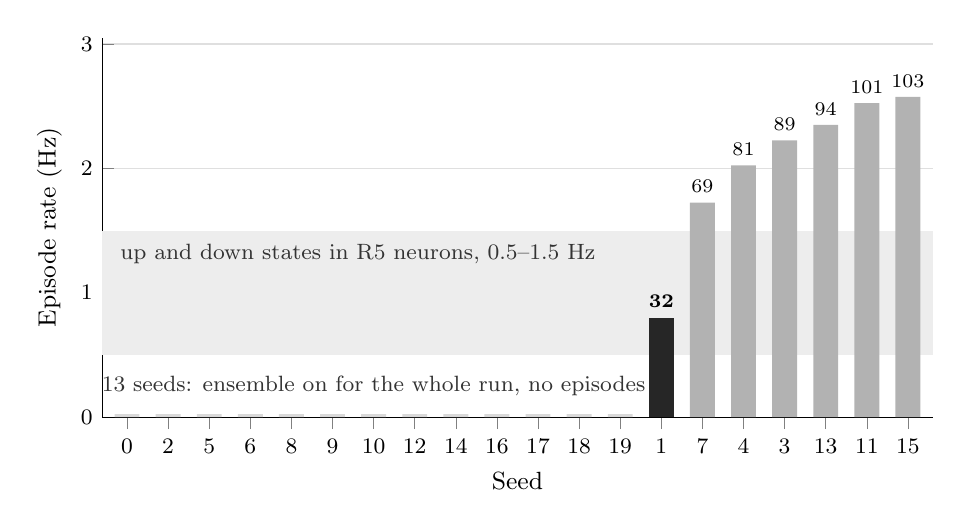
\begin{tikzpicture}
\begin{axis}[
  width=\textwidth, height=6.4cm,
  ybar, bar width=9pt, bar shift=0pt,
  ymin=0, ymax=3.05, xmin=0.4, xmax=20.6,
  ylabel={Episode rate (Hz)}, ylabel style={font=\small},
  xlabel={Seed}, xlabel style={font=\small},
  xtick={1,...,20},
  xticklabels={0,2,5,6,8,9,10,12,14,16,17,18,19,1,7,4,3,13,11,15},
  ytick={0,1,2,3},
  tick label style={font=\footnotesize},
  axis x line*=bottom, axis y line*=left,
  ymajorgrids, grid style={draw=gray!25},
  enlarge x limits=false,
  clip=false,
]
  \fill[gray!14] (axis cs:0.4,0.5) rectangle (axis cs:20.6,1.5);
  \node[anchor=north west, font=\footnotesize, text=quiet] at (axis cs:0.6,1.47) {up and down states in R5 neurons, 0.5--1.5 Hz};
  % 13 seeds on for the whole run (one 40 s episode = 0.025 Hz)
  \addplot[fill=gray!30, draw=none] coordinates {(1,0.025) (2,0.025) (3,0.025) (4,0.025) (5,0.025) (6,0.025) (7,0.025) (8,0.025) (9,0.025) (10,0.025) (11,0.025) (12,0.025) (13,0.025)};
  % seeds that burst outside the band
  \addplot[fill=gray!60, draw=none] coordinates {(15,1.725) (16,2.025) (17,2.225) (18,2.35) (19,2.525) (20,2.575)};
  % the one seed inside the band
  \addplot[fill=accent, draw=none] coordinates {(14,0.8)};
  % episode counts above bars
  \node[anchor=south, font=\scriptsize\bfseries] at (axis cs:14,0.8) {32};
  \node[anchor=south, font=\scriptsize] at (axis cs:15,1.725) {69};
  \node[anchor=south, font=\scriptsize] at (axis cs:16,2.025) {81};
  \node[anchor=south, font=\scriptsize] at (axis cs:17,2.225) {89};
  \node[anchor=south, font=\scriptsize] at (axis cs:18,2.35) {94};
  \node[anchor=south, font=\scriptsize] at (axis cs:19,2.525) {101};
  \node[anchor=south, font=\scriptsize] at (axis cs:20,2.575) {103};
  \node[font=\footnotesize, text=quiet, align=center] at (axis cs:7,0.25) {13 seeds: ensemble on for the whole run, no episodes};
\end{axis}
\end{tikzpicture}
\caption{Only 1 of 20 seeds bursts inside the band measured in flies. Bars show the trained ensemble's episode rate in each 40~s sleep run with adaptation ($\tau = 200$~ms, $b = 0.5$~mV); numbers above bars are episode counts. Seeds on the left had one continuous episode for the whole run. Band from \citet{raccuglia2019}.}
\label{fig:census}
\end{figure}

\paragraph{Measured short-term depression removes the runaway, and the mushroom-body activity with it.} The one slow mechanism whose magnitude is measured is depression at antennal-lobe synapses, fit three times, onto two postsynaptic cell types. What is not measured is which synapses to apply it to, so scope was an arm and all nine runs (three fits $\times$ three scopes) are reported. Where it was measured, at receptor-neuron synapses, it does nothing: local interneurons still fire at 126.6~Hz, because offline there is no odour and those synapses carry almost no traffic. Extrapolated to the antennal-lobe loop, it works as predicted before the runs: the local interneurons fall to between 0.2 and 3.8~Hz, and Kenyon-cell activity falls with them, from 0.43 to 0.003~Hz, a factor of about 140. The offline Kenyon-cell activity measured in every earlier stage was therefore the antennal-lobe runaway driving it; with the runaway gone there is nothing left in the mushroom body to reactivate. Under the sparsity floor, no run produced an episode in the brain or the ensemble.

\paragraph{A slow afterhyperpolarisation on APL, first run.} \citet{chen2026} recorded an SK-channel afterhyperpolarisation on APL with a decay constant of $491.1 \pm 72.2$~ms, enhanced by sleep deprivation and reduced by recovery sleep; the same recordings independently confirm that APL is non-spiking. On APL this term would release the mushroom body's gain control with a lag of about half a second, shorter than the 0.67 to 2~s period implied by the measured up-state band. Its amplitude is not measured. So far only a 3~s smoke run exists, at the measured $\tau$, one gain and one seed, and it produced no episode. The planned scan over gain and over the edges of $\tau$'s error bar has not been run, so this mechanism is untested rather than rejected.

% =====================================================================
\section{Discussion}

\paragraph{The negative is architectural.} The memory in this model is a depression of \KCMBON{} synapses, one stage downstream of the Kenyon cells whose reactivation is scored (Figure~\ref{fig:circuit}). Learning can change what the mushroom body sends, and it does: offline drive through the learned synapses falls by a third. It cannot change which Kenyon cells switch on unless the change travels back. The only return path that prefers the trained ensemble delivers under 1\% of a threshold gap even at 50~Hz, and its source is silenced by APL in 19 of 20 seeds. Adding episodes did not alter this, because episodes do not move the engram. In this model class a positive Kenyon-cell replay result would have to be explained by something other than the memory.

\paragraph{A model can pass its benchmark and still be wrong elsewhere.} The published model reproduces its gustatory benchmark closely, and this reimplementation matches it. Yet in olfaction it codes odours with more than half of all Kenyon cells, because APL is given a threshold it does not have: inhibition that should be continuous arrives in pulses that Kenyon cells can fire between. The benchmark could not reveal this, because the 21-neuron gustatory stimulus never ignites the network. Whole-brain models are validated pathway by pathway, and a non-spiking cell modelled as spiking can be invisible in every pathway but its own.

\paragraph{Measured values beat fitted ones here.} Both corrections, and the depression constants, came from recordings on identified cells and added no parameters. The APL correction alone moved the code onto the measured sparseness. By contrast, the natural global knob, scaling every weight down, only silenced the Kenyon cells before it stopped the runaway. The pattern suggests that the errors in connectome models are often in cell-type physiology and transmitter assignment rather than in global constants.

\paragraph{What a replay-capable model would need.} The measurements point to four requirements. First, a slow variable that ends an up state; the published model has nothing slower than 20~ms. Second, a background that pauses rather than a runaway, which here means resolving why antennal-lobe local interneurons are 73\% excitatory onto each other under the sign rule. Third, plasticity at or upstream of the Kenyon cells, or a return path strong enough to carry the engram back. Fourth, an APL that does not silence the readout, for which the connectome already provides a parameter-free partition into 36 neuropil compartments. A sleep manipulation that changes more than 0.2\% of brain activity would also be needed for the sleep-against-wake comparison to mean anything.

\paragraph{The tonic trace is the model's real offline memory signal.} The engram is expressed continuously, amplified about 26 times relative to the weight change, because offline activity falls disproportionately on the synapses that conditioning depressed. This is not replay by any of the criteria used here. It is, however, a concrete form in which a downstream engram can be present during sleep without any ensemble reactivating. Whether flies show an analogous offline shift in MBON input is an open question that this model raises but cannot settle.

\paragraph{Method.} Three choices decided the interpretation. The unlearned-weights control, not one of the four pre-registered comparisons, was the only test that asked whether the memory contributed anything. Arm matching exposed that two of the four comparisons set networks in different states against each other. And the positive control showed that, without a slow variable, no detector could have found replay, so the first negative could not be read as evidence of absence. A census across all 20 seeds then corrected a three-seed impression that episodes were typical.

\section{Limitations}
The model inherits the simplifications of the published one, and this project adds a few of its own.
\begin{itemize}\setlength\itemsep{1pt}
  \item \textbf{Point neurons with uniform biophysics.} Every cell is one compartment with the same membrane time constant, threshold and refractory period, whatever its type or size. There is no dendritic processing and no morphology, and conduction delay is a single constant.
  \item \textbf{Predicted transmitters.} Synaptic signs come from a machine-learning prediction on synapse images. Two were corrected here; others, including those of the antennal-lobe local interneurons, may be wrong. The 952 neurons with no prediction default to excitatory without a source.
  \item \textbf{One plasticity locus.} Only \KCMBON{} synapses can change, which the Discussion identifies as the main reason the test cannot come out positive.
  \item \textbf{Unmeasured constants.} The DAN pairing rate (20~Hz), the gating threshold of 5 DAN$\rightarrow$MBON synapses, the dFB clamp rate (17~Hz) and the background noise have no direct measurement, and the learning rate is fitted. Each is flagged in the project's parameter table.
  \item \textbf{Sampling of the deviations.} The adaptation and depression scans used one seed per setting; only the re-run replay test used 20. The APL afterhyperpolarisation has a single 3~s smoke run.
  \item \textbf{A male brain, no body.} Much of the calibration physiology was measured in females. The ventral nerve cord is excluded, and there is no behaviour or sensory feedback.
  \item \textbf{No event detector and no ground truth.} The fly has no described ripple analogue to trigger on, and offline reactivation of Kenyon-cell ensembles has never been observed in a real fly, so a positive result would have had no measurement to compare against.
  \item \textbf{The slow-wave band is not a sleep recording.} The 0.5 to 1.5~Hz band of R5 up and down states \citep{raccuglia2019} was measured in head-fixed flies and in explant brains, where its power rises over the day and after sleep deprivation; it was not recorded in flies shown to be asleep. \citet{raccuglia2025} use the same band. It serves here as the nearest measured timescale for up and down states in the fly.
\end{itemize}

\section{Conclusion}
A whole-brain connectome model of \Dm{}, corrected where direct measurements contradict it, does not replay a learned Kenyon-cell ensemble during simulated sleep. The answer holds at published parameters and in a deviated model that can hold episodes and codes odours at a realistic sparseness. The reason is structural: the engram sits downstream of the cells being scored, and the path back is too weak to carry it. The memory is still present offline, as a continuous 32.5\% reduction in drive through the learned synapses. Testing Kenyon-cell replay in this framework needs plasticity at or upstream of the Kenyon cells, a slow variable, and an antennal lobe that does not run away. Until then, the negative is a fact about the model, not about the fly.

\section*{Code and Data Availability}
\addcontentsline{toc}{section}{Code and Data Availability}
Code, configurations and result files are in the hypnagogia repository (\url{https://github.com/ankthba/hypnagogia}). Each stage named in this paper is one script under \texttt{scripts/}, with its outputs under \texttt{results/}; the base configurations are under \texttt{configs/}. The summary file \texttt{results.md} is generated from those outputs by the script \texttt{scripts/make\_results.py}. The male CNS v1.0 tables and FlyWire v630 and v783 are fetched by \texttt{scripts/fetch\_data.py}. The model runs on Brian2 2.10.1 in C++ standalone mode.

\section*{Acknowledgments and Use of AI Tools}
\addcontentsline{toc}{section}{Acknowledgments and Use of AI Tools}
This work was developed with Anthropic's Claude as a collaborator on the code, the analysis and the writing. Any errors are the author's own.

\bibliographystyle{plainnat}
\bibliography{references}

\end{document}
